\documentclass{article}
\usepackage{listings}
\usepackage{ctex}
\usepackage{graphicx}
\usepackage[a4paper, body={18cm,22cm}]{geometry}
\usepackage{amsmath,amssymb,amstext,wasysym,enumerate,graphicx,caption,subfigure}
\usepackage{float,abstract,booktabs,indentfirst,amsmath}
\usepackage{array}
\usepackage{booktabs} %调整表格线与上下内容的间隔
\usepackage{multirow}
\usepackage{url}
\usepackage{diagbox}
\renewcommand\arraystretch{1.4}
\usepackage{indentfirst}
\setlength{\parindent}{2em}
\usepackage{listings}
\usepackage{xcolor}
\lstset{
	numbers=left, 
	numberstyle= \tiny, 
	keywordstyle= \color{ blue!70},
	commentstyle= \color{red!50!green!50!blue!50}, 
	frame=shadowbox, % 阴影效果
	rulesepcolor= \color{ red!20!green!20!blue!20} ,
	escapeinside=``, % 英文分号中可写入中文
	xleftmargin=2em,xrightmargin=2em, aboveskip=1em,
	basicstyle=\footnotesize,
	framexleftmargin=2em
} 


\geometry{left=2.8cm,right=2.2cm,top=2.5cm,bottom=2.5cm}
%\geometry{left=3.18cm,right=3.18cm,top=2.54cm,bottom=2.54cm}

\graphicspath{{figures/}}

\title{\heiti 数字电路实验报告 }

\begin{document}
	\vspace*{1cm}
	
	\begin{figure}[h]
		\centering
		
\includegraphics[scale=1.0]{xh.jpg}
	\end{figure}

	\vspace*{0.5cm}
	
	\begin{center}
		\Huge{\textbf{数字电路实验报告}}
	\end{center}
	
	\vspace{5cm}
	
	\begin{table}[h]
		\centering
		\begin{Large}
			\begin{tabular}{p{3cm} p{7cm}<{\centering}}
				实验题目: &   综合实验     \\ \cline{2-2}
				学生姓名:      & 孔浩宇   \\ \cline{2-2}
				学生学号: & PB20000113 \\ \cline{2-2}
				完成日期:       & 2022/12/14 \\ \cline{2-2}
			\end{tabular}
		\end{Large}		
	\end{table}
	\newpage
    \section{实验题目}
        \subsection*{\qquad  综合实验}
     
    \section{实验目的}
        \begin{enumerate}
            \item [1.]熟练掌握前面实验中的所有知识点
            \item [2.]熟悉几种常用通信接口的工作原理及使用
            \item [3.]独立完成具有一定规模的功能电路设计
        \end{enumerate}

    \section{实验环境}
        \subsection*{\qquad (1) Logisim}
        \subsection*{\qquad (2) vscode}
        \subsection*{\qquad (3) python 3.11}
        \subsection*{\qquad (4) c++}
    
	\clearpage
    \section{实验练习}
	\subsection{程序实现的功能}
	输入汉字,实现机内码到机位码的转化,存储在 ROM 内,
	自动生成 logisim电路,实现汉字的滚动或闪烁显示

	\subsection{设计思路}
	\subsubsection{汉字转化部分}
	在 GB2312 编码中,一个汉字用两个字符表示,可以在对应的 HZK16 的字
	库获得其 16*16 的表示,具体实现为根据字符计算 offset,然后根据
	offset 查找对应的二进制表示,具体代码实现如下,输入为一个汉字,
	返回一 01 字符串:

	\begin{figure*}[htbp]
		\centering
		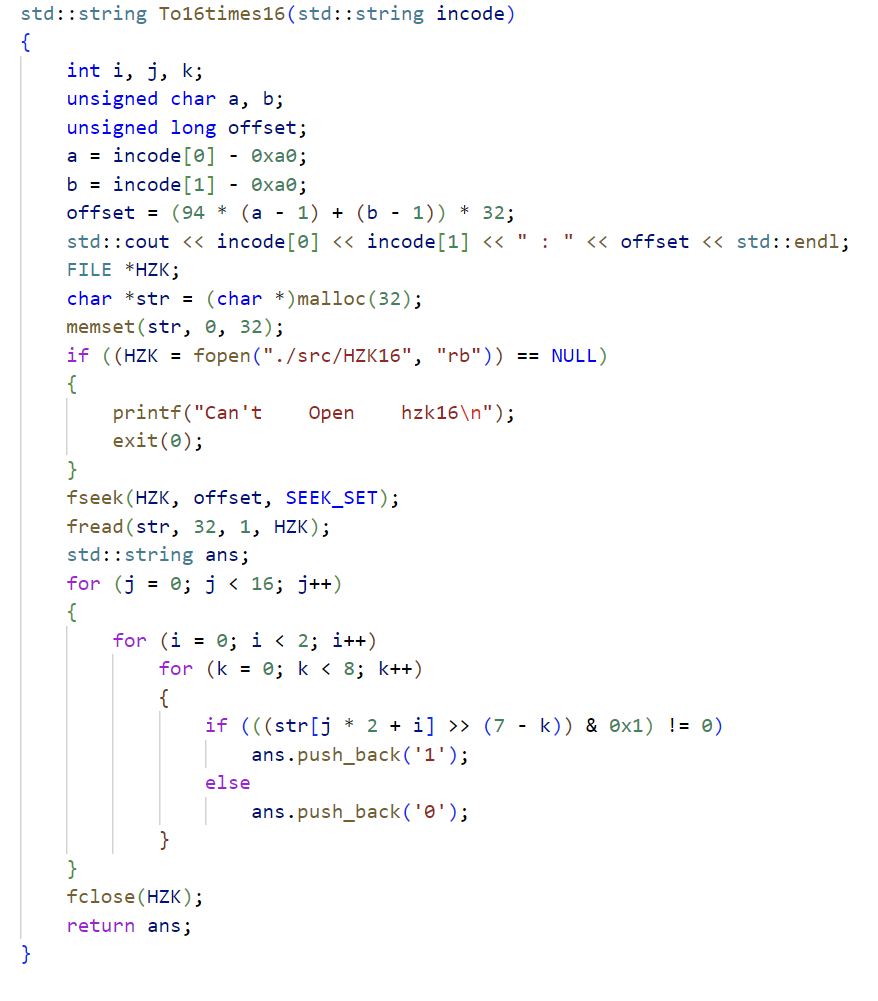
\includegraphics[scale=0.8]{to16.png}
	\end{figure*}

	\clearpage
	\subsubsection{转化为ROM的值}
	Logisim 生成的.circ 文件是一 xml 语言书写的文件,可以通过修改对应
	label 的值,来改变 ROM 的值,同时存储的 ROM 值是十六进制形式,所
	以需要将获得的汉字对应的二进制字符串转化为十六进制,如下为一将
	256 位二进制字符串转化成 16 进制的函数
	
	\begin{figure*}[htbp]
		\centering
		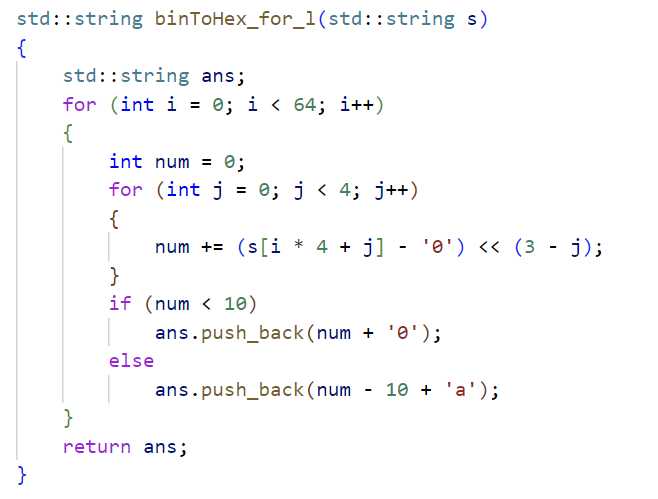
\includegraphics[scale=0.8]{bfl.png}
	\end{figure*}

	\subsubsection{生成电路}
	输入汉字全部转化成十六进制字符串后,首先从文件读入.circ 文件基本的信息,
	\begin{figure*}[htbp]
		\centering
		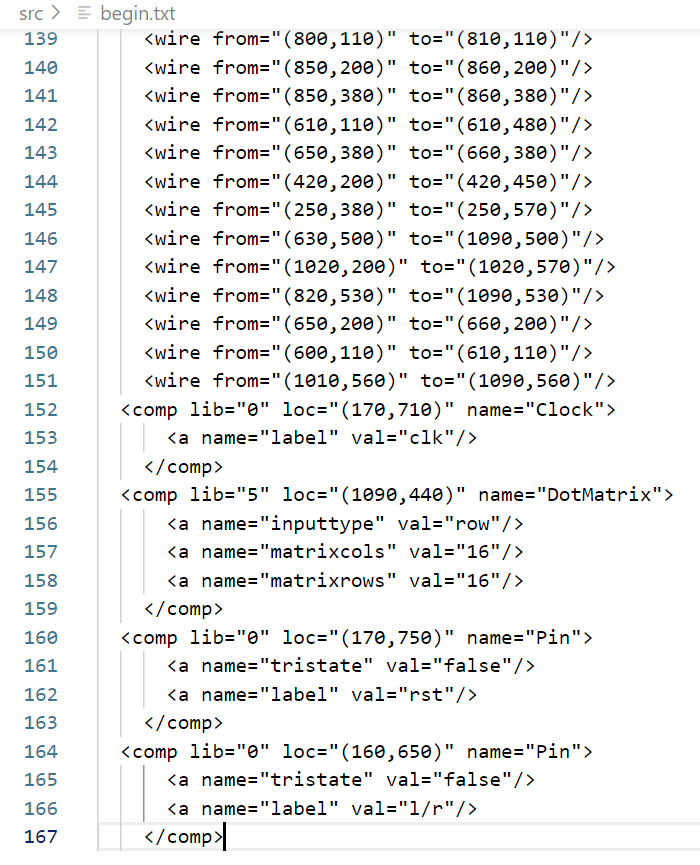
\includegraphics[scale=0.7]{begin.png}
	\end{figure*}

	接着,将对应的 ROM 输出
	\begin{figure*}[htbp]
		\centering
		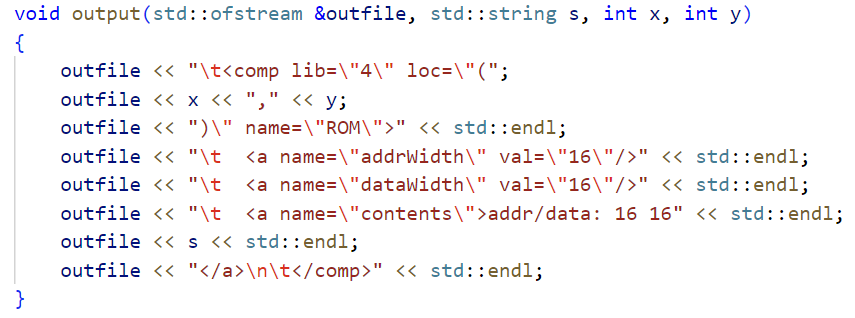
\includegraphics[scale=0.8]{output.png}
	\end{figure*}
	
	\subsubsection{计数器的最大值更改}
	根据所需生成画面的总数,直接修改 counter 的最大值,以 std::hex的格式输出
	\begin{figure*}[htbp]
		\centering
		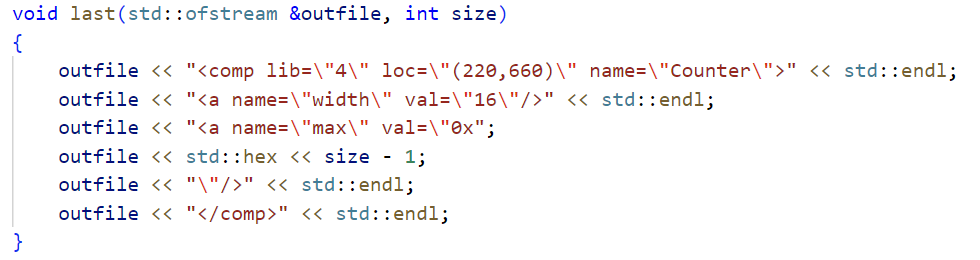
\includegraphics[scale=0.8]{counter.png}
	\end{figure*}

	\subsubsection{滚动画面的实现}	
	闪烁显示时,一个时钟周期显示一个汉字,滚动显示则将下一个汉字逐
	步显示出来,每一个时钟周期,移动一个 bit

	\subsubsection{用户交互}
	交互部分通过 python 脚本,编译运行 cpp 程序,并通过 logisim 打开输出文件
	\begin{figure*}[htbp]
		\centering
		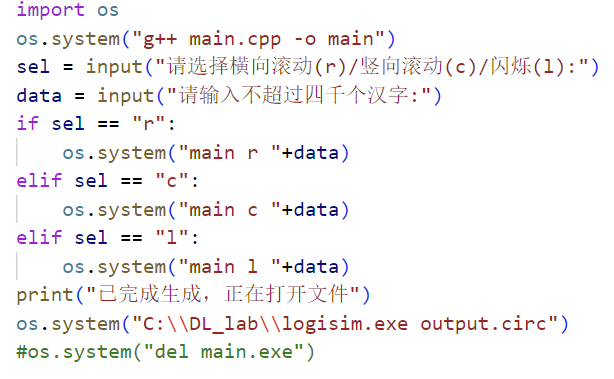
\includegraphics[scale=0.8]{py.png}
	\end{figure*}

	\clearpage
	\subsection{运行效果}

	\begin{figure*}[htbp]
		\centering
		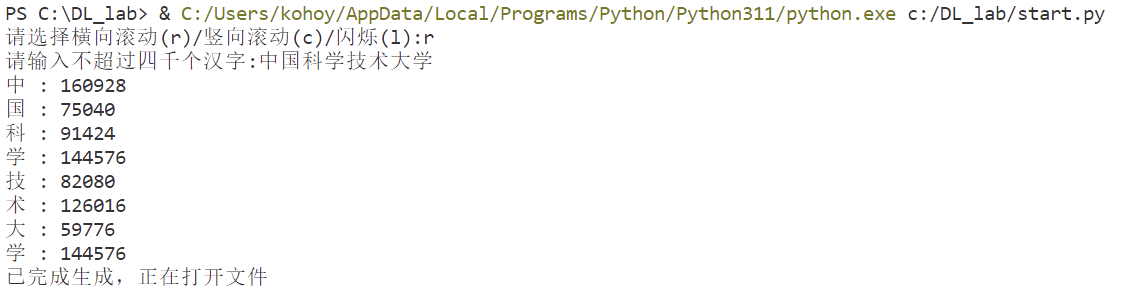
\includegraphics[scale=0.8]{op.png}
	\end{figure*}

	\begin{figure*}[htbp]
		\centering
		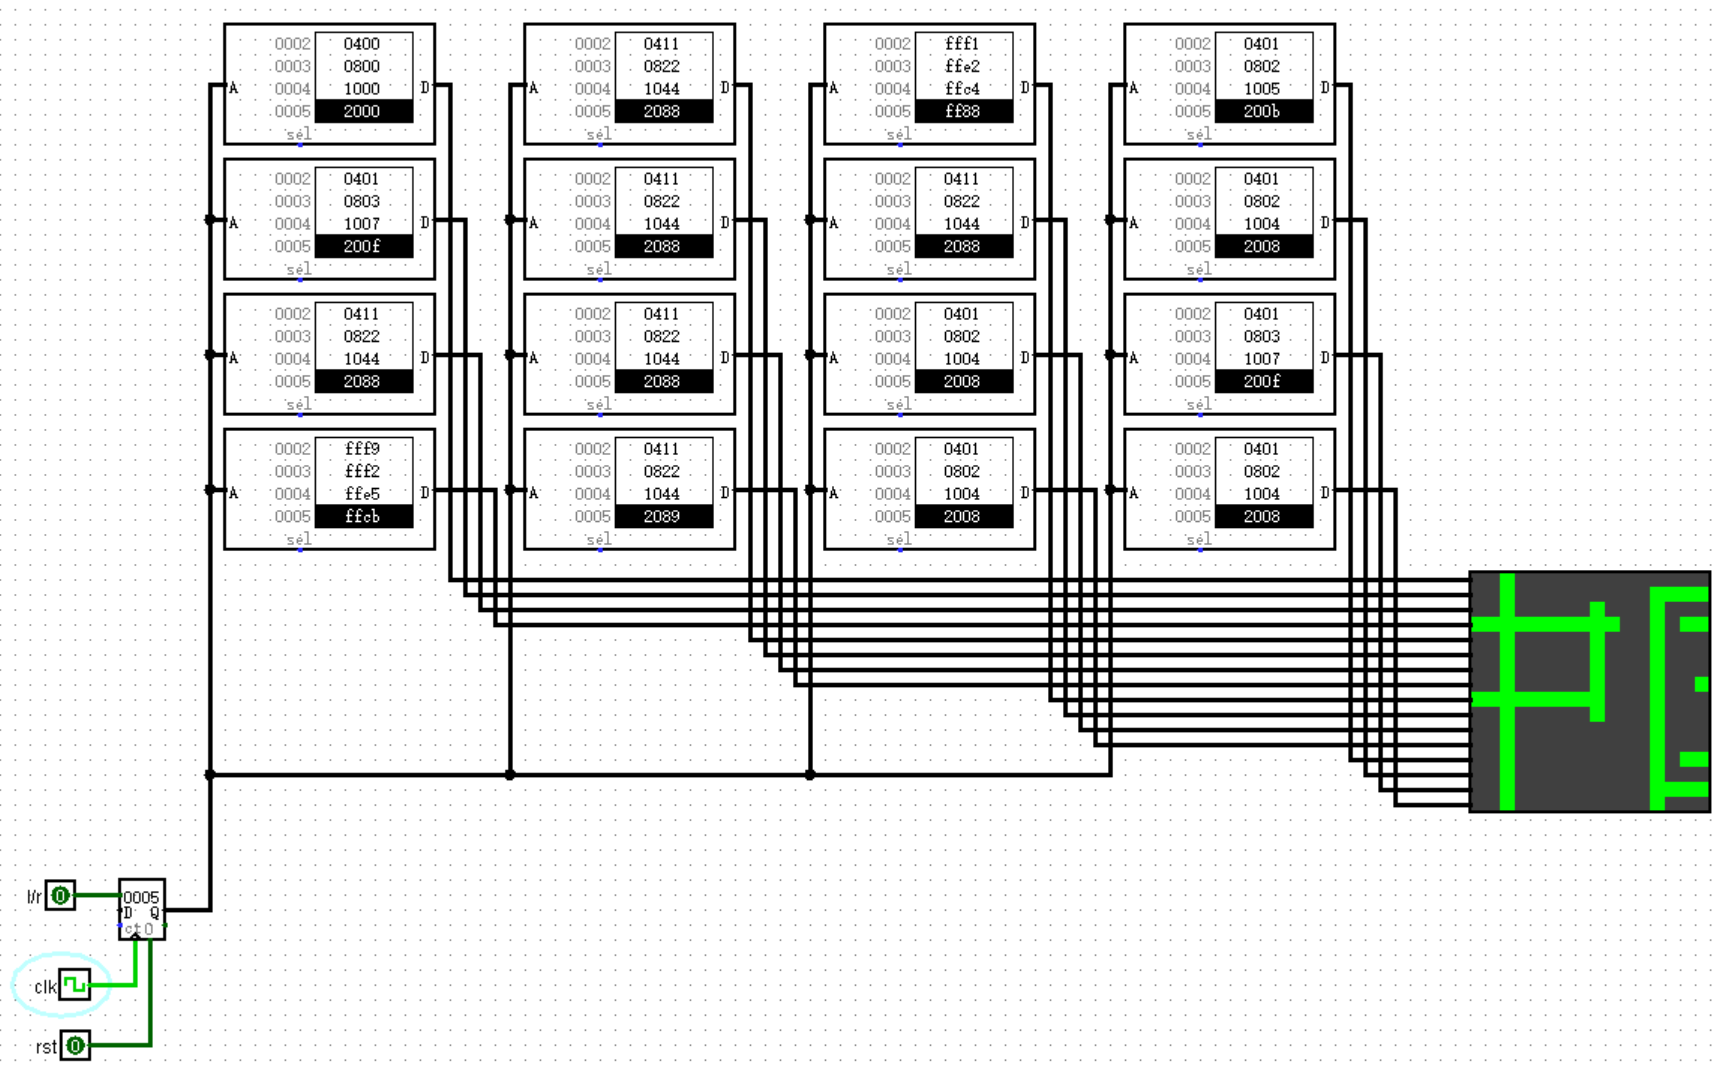
\includegraphics[scale=0.4]{re.png}
	\end{figure*}


	\subsection{程序稳定性及可扩展性}
	\begin{enumerate}
		\item [1.]程序可实现上千汉字的转化,仍然可以稳定运行
		\item [2.]利用修改 xml 文件的方法,不仅仅可以修改 ROM,还可以生成逻辑电路,
		稍加修改之后,可以实现基本的可编程逻辑电路的功能
	\end{enumerate}

    \section{总结与思考}
	\begin{enumerate}
		\item [1.]通过本实验熟悉了机内码到区位码的转换,对逻辑电路有了更深的认识
		\item [2.]本次实验较难
		\item [3.]本实验共用时约四个小时,共编写了两百余行代码,任务量较大
		\item [4.]无建议
	\end{enumerate}
\end{document}